\documentclass[hyperref, UTF8, cs4size, titlepage]{ctexart}

% 版面制作
\usepackage[a4paper, left=2.5cm, right=2.5cm, top=2.5cm, bottom=2.5cm]{geometry}
% 页面(页尾设置)
\pagestyle{plain}

% 目录拓展
\usepackage[nottoc]{tocbibind}
% 超文本链接设置
\usepackage{bookmark}
\hypersetup{colorlinks=true, linkcolor=blue, filecolor=magenta, urlcolor=cyan, pdfpagemode=FullScreen}

% 引用设置
\bibliographystyle{plain}
% 索引设置
\usepackage{makeidx}
\makeindex
% 附件添加
\usepackage{attachfile}

% 标题设置
\usepackage[raggedright]{titlesec}
\titleformat*{\section}{\large\upshape\bfseries\centering}
% 行距设置
%\usepackage{setspace}
%\singlespacing

% 数学
\usepackage{amsmath}

% 图表
\usepackage{caption} % 图表标题
\usepackage{graphicx} % 图片
\usepackage{booktabs} % 三线表

% 自定义命令
\newcommand{\keywords}[1]{\textbf{\textit{关键字---}} #1}

\begin{document}

  % 添加封面
  \begin{titlepage}
  \begin{center}
    \vspace*{\fill}
    {\zihao{3}\bfseries 选题:A}
    \vspace*{\fill}

    {\zihao{3}\bfseries 论文题目:}
    \vspace*{\stretch{2}}

    \zihao{4}\itshape
    \begin{tabular}{ccc}
      建模:& 成宇琛 & 电气 1813 班 \\
      编程:& 孙瑞 & 计算机 1806班 \\
      论文:& 邓思彤 & 电气 1813 班 \\
    \end{tabular}
    \vspace*{\stretch{3}}

    \today
  \end{center}
  \vspace*{\stretch{1}}
\end{titlepage}

  % 添加摘要
  \phantomsection
  \begin{abstract}
  \thispagestyle{plain}

  碳排放问题在我国已引起广泛的关注。为对我国实施碳排放减排政策和低碳经济发展战略提供决策依据和有效建议。现对外来几年的碳排放进行预测,并以此提供有效建议。

  \textbf{针对问题一:}
  
  本文做出了了煤炭、石油、天然气和一次电力及其他能源占我国能源消费整体的比重随年份变化的折线图。

  以此为依据展开对我国能源消费结构的分析。分析包括了沿y轴(能源所占比例)和沿x轴(年份变化)的大小与趋势的分析。

  最终得出了:我国能源结构以化石能源(煤炭尤其)为其始终主导的现状;和总体能源结构在不断优化,但仍有相当大发展空间的未来趋势。

  \textbf{针对问题二:}
  
  本文选取、整理了总人口数、$\mathrm{GDP}$、产业结构、城镇化率、经济发展水平、国际贸易、人均碳排放量、能源消费强度,共八个因素作为主要影响因素,并以此建立了\textbf{ $\mathrm{BP}$ 神经网络模型}。

  具体来说:

  本文首先对样本数据进行计算、分类和归一化处理。再确定模型输出层、中间隐层和输入层,以及具体函数、参数选取、初始化。

  之后借助于 $\mathrm{MATLAB}$ 软件中的神经网络计算功能,对模型进行了合理训练和数据拟合。最终得到对应年份的碳排放量的模拟值和预测值。

  \textbf{针对问题三:}
  
  本文首先在\emph{模型评价与改进}中应用\textbf{关联度分析法}建立了\textbf{灰色关联模型}。
  
  之后代入数据到关联系数公式中,得出影响因素数列对参考数列的关联度,以此对各影响因素进行了关联性排序。

  通过关联度大小排序也就得到了影响因素的重要性排序。其结果是:$\text{总人口数}>\mathrm{GDP}>\text{其他}$。其中,总人口数和$\mathrm{GDP}$ 关联度徘徊在 0.6 上下,其他值集中在 0.39 上下。

  最终我们根据影响因素的重要性,提出:
  \begin{enumerate}
    \item 加快中国 $\mathrm{GDP}$ 由高速度增长向高质量发展的经济转型。
    \item 坚持计划生育的基本国策。
    \item 转移城市过剩生产力,帮助农村发展,减少城乡差异。
    \item 寻求开发绿色能源、新能源,减少对化石能源的依赖。
  \end{enumerate}

  \vspace{\stretch{3}}
  {\keywords{碳排放,能源结构,$\mathrm{BP}$ 神经网络,灰色关联模型,关联度分析法}}
  \vspace{\fill}
\end{abstract}
  \addcontentsline{toc}{section}{摘要}
  \clearpage

  % 添加目录
  %\phantomsection
  \tableofcontents
  \thispagestyle{empty}
  \clearpage

  % 内容

  \section{问题重述}

  \subsection{问题背景}

  \subsection{问题提出}
  \clearpage

  \section{问题分析}

  \subsection{问题 1:我国能源结构分析}

    我们将煤炭、石油、天然气和一次电力及其他等能源占能源消费总量的比重,按时间序列作出折线图(见图 \ref{fig:nenyuanxiaofeibizhong})。
    \begin{figure}[hb]
      \centering
      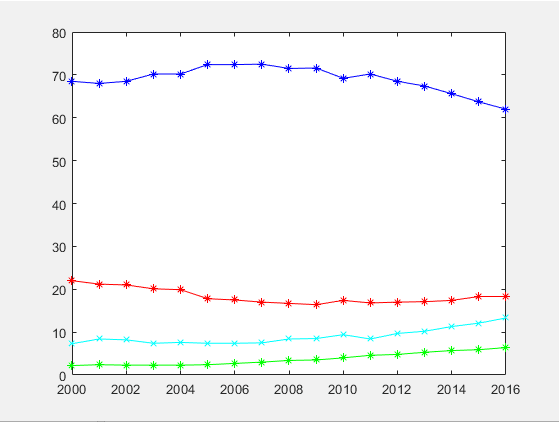
\includegraphics[scale=0.6]{figures/fig1.png}
      \captionsetup{format=hang}
      \caption[煤炭、石油、天然气和一次电力及其他等能源占能源消费总量的比重]{蓝色曲线为煤炭占总能源的比例,红色为石油,绿色为天然气,青色为一次电力及其他能源。}
      \label{fig:nenyuanxiaofeibizhong}
    \end{figure}

    由图 \ref{fig:nenyuanxiaofeibizhong} ,沿 $y$ 轴可以分析出以下几点:
    \begin{enumerate}
      \item 煤炭消费占我国能源消费的首要地位,其比例始终居于 $60\%$ 之上。
      \item 石油消费为最主要的辅助能源,其比例一直在 $20\%$ 附近。
      \item 一次电力能源与天然气在总能源中的比例相对较低,大体上低于 $10\%$ 。
    \end{enumerate}

    再沿时间轴可以分析出:
    \begin{enumerate}
      \item 煤炭消费在波动中整体呈现缓步下降趋势,但仍然占据我国能源消费的首要地位。
      \item 石油消费在参考年限中呈稳定趋势,略有波动和下滑。但与一次电力及其他的距离不断拉近。
      \item 一次电力及其他能源和天然气能源消费是呈逐年上升趋势,且天然气的上升速度随年份增加而增加。但所占比例仍然不足。
    \end{enumerate}

    \subsubsection{总结}
    我国的能源消费结构始终为以煤炭消费为主导地位,并以石油消费为主要辅助消费,但也存在天然气、一次电力及其他能源等能源占据市场。能源消费市场呈现 “一超多强” 局面。
    
    天然气和一次电力这样的清洁能源与石油、煤炭消费所占的比重不断拉近,但仍未占据可观消费比例。这说明我国的能源消费结构在不断优化的过程中还有很大的发展空间。

  \subsection{问题 2:碳排放预测模型}

    \subsubsection{碳排放影响因素分析}
      为建立模型,需要对碳排放的影响因素进行分析。根据有关文献,碳排放影响因素一般包括:
      \begin{enumerate}
        \item 人口因素;
        \item 城镇化率;
        \item 经济发展水平:人均 $GDP$ 或者消除价格波动影响的国内生产总值;
        \item 人均碳排放量;
        \item 能源消费强度:能源消费量与 $GDP$ 之比;
        \item 能源消费结构:各种能源所占比例,可以用煤炭比例来表示;
        \item 产业结构:三类产业占比,可以用第二产业占比表示;
        \item 国际贸易:出口额占 $GDP$ 比重。
      \end{enumerate}
      我们选取% TODO 因素
      进行分析。
    
    \subsubsection{模型建立}
      我们用多云线性回归分析对上述选取的因素建立了模型。

  \subsection{问题 3:政策建议}
    参见 \hyperref[sec:zhencejianyi]{7 政策建议}。
  \clearpage

  \section{模型假设}

  \section{符号说明}
  \begin{table}[hb]
    \caption{符号说明}
    \label{tab:fuhaoshuoming}
    \centering
    \begin{tabular}{cc}
      \toprule[1.5pt]
      符号 & 说明 \\
      \midrule[1pt]
      $Y$ & 碳排放总量 \\
      $X1$ & 总人口数 \\
      $X2$ & $GDP$ \\
      $X3$ & 产业结构 \\
      $X4$ & 城镇化率 \\
      $X5$ & 经济发展水平 \\
      $X6$ & 国际贸易 \\
      $X7$ & 人均碳排放量 \\
      $X8$ & 能源消费强度 \\
      \bottomrule[1.5pt]
    \end{tabular}
  \end{table}

  \section{模型建立及求解}
  \clearpage

  \section{模型评价与改进}

  \section{政策建议}
  \label{sec:zhencejianyi}

  \subsection{建议一}
    我们根据\emph{模型评价与改进}中的灰色预测模型得到了影响因素的重要性排序。结果:
    \[
      \text{总人口}>\textrm{GDP}>\text{其他因素}
    \]
    可见\textbf{总人口}和 \textbf{GDP} 对碳排放量影响最大,其他影响因素之间相差无几。
    
    在其中,\textbf{总人口}一定程度上代表全部人口需要的生产物资、\textbf{GDP} 代表全年所有商品生产的价值总和。需要生产的产品越多,所消耗的能源也越多,因此碳排放量也就越大。
    
    在改革不能自己把自己革命了的前提下,我们提出:
    \begin{enumerate}
      \item 坚持计划生育的基本国策。
      \item 加快中国 $\mathrm{GDP}$ 由高速度增长向高质量发展的经济转型;去杠杆、降产能,稳中求进,积极转变。
      \item 转移城市过剩生产力,帮助农村发展,减少城乡差异;精准扶贫,建设全面小康。
    \end{enumerate}

  \subsubsection{建议二}
    另外,碳排放量在能源消耗一定的情况下,与能源结构、能源利用率有较大关联。
    因此我们提出:
    \begin{enumerate}
      \item 提高化石能源利用率,关闭一些高耗能、高污染、技术落后的小、中型发电厂,加快新技术的研发和推广。
      \item 积极推广绿色能源(风电、水电等)、积极研发新能源,减少对化石能源的依赖。
    \end{enumerate}
  \clearpage

  % 引用文献
  \phantomsection
  \bibliography{ref/math_model.bib}
  \clearpage

  % 索引
  \phantomsection
  \printindex

  % 附录
  \appendix

  \section{附件 1}
    中国近些年来的一些经济数据\footnote{来源:中国统计年鉴及中国能源统计年鉴}。
    \attachfile{appendix/fujian1.xlsx}
    \label{sec:fujian1}

  \section{附录 2}

\end{document}